\section{Plannung}

\subsection{Ideenfindung [M]}
\setauthor{Fabian Maar}
Die Ideenfindung ist der Start eines Projektes und bildet das Fundament, auf dem das Projekt entsteht. Die Idee für die Entstehung eines Projektes kann viele Motive haben, so ist es wichtig, als Projektteam diese zu erkennen und als Motivation zu nehmen. Während oder nach dem Prozess der Ideenfindungs wird schon bald klar, welche Projektwürdigkeit das Projekt besitzt. Somit kann schon frühzeitig entschieden werden, ob es sinnvoll erscheint, das Projekt zu realisieren oder ob nochmals eine neue Ideenfindung von Nöten ist. Auch bei dieser Diplomarbeit wurde der Prozess der Ideenfindung mehrmals wiederholt, wodurch die Wichtigkeit und die Methodik der Findung von Ideen besonders bemerkbar wurde. Die Ideenfindung erfolgt meist mit Hilfe der Anwendung einer passenden Kreativitätstechnik.

Kreativitätstechniken sind vielseitig einzusetzen, werden aber häufig am Anfang eines Projektes angewandt. Sie sind besonders hilfreich, wenn ein rationales Problemlösen nicht zielführend erscheint. Sie helfen, Ziele, Lösungen und Risiken zu finden, evaluieren und festzulegen. Für die Diplomarbeit bot sich besonders die Kreativitätstechnik Brainstorming an, da durch sie viele verschiedene Ideen in kürzester Zeit gesammelt werden können.

Beim Brainstormen findet jede*r Teilnehmer*in zu einem bestimmten Thema so viele Ideen wie möglich. Das Brainstormen erfolgt in 2 Phasen. Zuerst werden alle Ideen niedergeschrieben und anschließend die Beste herausgefiltert. Aufgrund der Expertise der Betreuungslehrerinnen im Bereich 3D-Modellierung und aus eigenem Interesse, konnte sich relativ schnell auf das Thema \emph{eine Software mit 3D-Integration} geeinigt werden. Schlussendlich konnte sich für eine Idee entschieden werden, nachdem das Brainstormen nach folgenden Kriterien erfolgt hat:
\begin{itemize}
    \item Quantität vor Qualität
    \item Freies Assoziieren und Fantasieren sind erwünscht
    \item Keine Kritik, Korrektur oder Meinungsäußerung
    \item Möglichst viele Ideen
    \item Inspirieren lassen von anderen
\end{itemize}

\cite{Ideenfindung}

\subsection{fortlaufendes Prototyping}
\label{ch::ongoing-prototyping}

\section{Design}
\subsection{Userexperience [L]}
\setauthor{Litzlbauer Lorenz}
In keinem Softwareprojekt darf nicht der*die Benutzer*innen vergessen werden. Feature und Design müssen immer mit dem Gedanken entwickelt werden, wie hilft das dem*der Kunden*in oder der Zielgruppe weiter.

In den folgenden Kapiteln wird das Thema User Experience und wie dieses Thema im Projekt umgesetzt wurde, behandelt.
\subsubsection{UX Design (Userexperience)}
Ein gutes Userexperience-Design ist die Grundlage für eine erfolgreiche Positionierung und Kommunikation mit dem*der Benutzer*in.
UX bezieht sich dabei auf die Interaktion des Benutzers mit der Umwelt, aber auch mit dem angebotenen Service oder Produkt. In diesem Kontext hat Design mehrere Bedeutungen.
Erstens gibt es den Punkt der Gestaltung der Interaktionen, hierzu gehört der Begriff Interface Design (UI Design), er bedeutet visuelle Kommunikation über Zeichen und Symbole.
Zweitens gibt es Design als den Designprozess. Im Designprozess muss erkannt werden, was dem*der Benutzer*in wichtig ist und dieses dem Produkt zugewiesen werden, sodass es auch der*die Benutzer*in erkennen kann \cite{UserExperienceDesign}.

\subsubsection{Anwendungen von UX im Projekt}
Das Projekt wurde schon von Anfang an mit einem Gedanken für den Benutzer gestartet. Userstories waren aus der Sicht eines Benutzers formuliert und das Projekt startete mit der Frage, welchen Nutzen kann das Projekt einem*einer Nutzer*in geben.

Im Userinterface-Design wurde Figma (siehe Kapitel \hyperref[ch::technologies::figma]{Technologien Figma}) benutzt. Die Oberfläche wurde so designt, damit sie leicht verständlich, nützlich und benutzerfreundlich ist. Dafür wurden viele Prototypen (siehe Abbildung \ref{fig:impl:design:prototypesfigma}) in Figma gestallten und durch Umfragen die besten bestimmt und dementsprechende Anpassungen am Design gemacht.

\begin{figure}
    \centering
    \includegraphics[scale=0.3]{pics/ProjektOberflächenDesignPrototypenFigma.png}
    \caption{OberflächenDesign: Prototypen in Figma}
    \label{fig:impl:design:prototypesfigma}
\end{figure}

\subsection{Corporate Design [M]}
\setauthor{Fabian Maar}
Das Corporate Design unterstützt die Corporate Identity und deren Ziele. Unter der Corporate Identity versteht man das äußere Erscheinungsbild eines Unternehmens. Hierbei sollen Bestandteile eines Unternehmens nach außen hin einheitlich, unverwechselbar und positiv wirken und mit der Gesamtstrategie stimmig sein. Zum Beispiel werden Mitarbeiter, Abteilungen und Produkte sowie ihre Beziehungen zur Firma nach gewissen Normen strategisch gestaltet und geregelt. Dabei lässt sich die Corporate Identity in 3 Teilbereiche gliedern:

\begin{itemize}
    \item Corporate Behaviour
    \item Corporate Communication
    \item Corporate Design
\end{itemize}
\cite{CorporateIdentity}

Bei der Diplomarbeit kam vor allem das Corporate Design zum Einsatz. Hierbei wird vor allem das äußere Erscheinungsbild des Produkts als Einheit repräsentiert. Dabei werden zum Beispiel Hausfarbe, Logo, Gestaltungsraster und weitere Design-Elemente aufeinander abgestimmt. Dies war auch fester Bestandteil der Design-Phase.
\cite{CorporateDesign}

//TODO Text über Bild + Bilder richtig anordnen
Der erste Schritt des Designs war es, zwei unterschiedliche Konzepte der ersten Webseiten-Elemente zu erstellen. Anschließend wurden diese verglichen und sich für eines entschieden. Dieses erste Grundkonzept wurde das Grundgerüst für den späteren Verlauf der Designarbeit.

\begin{figure}
    \centering
    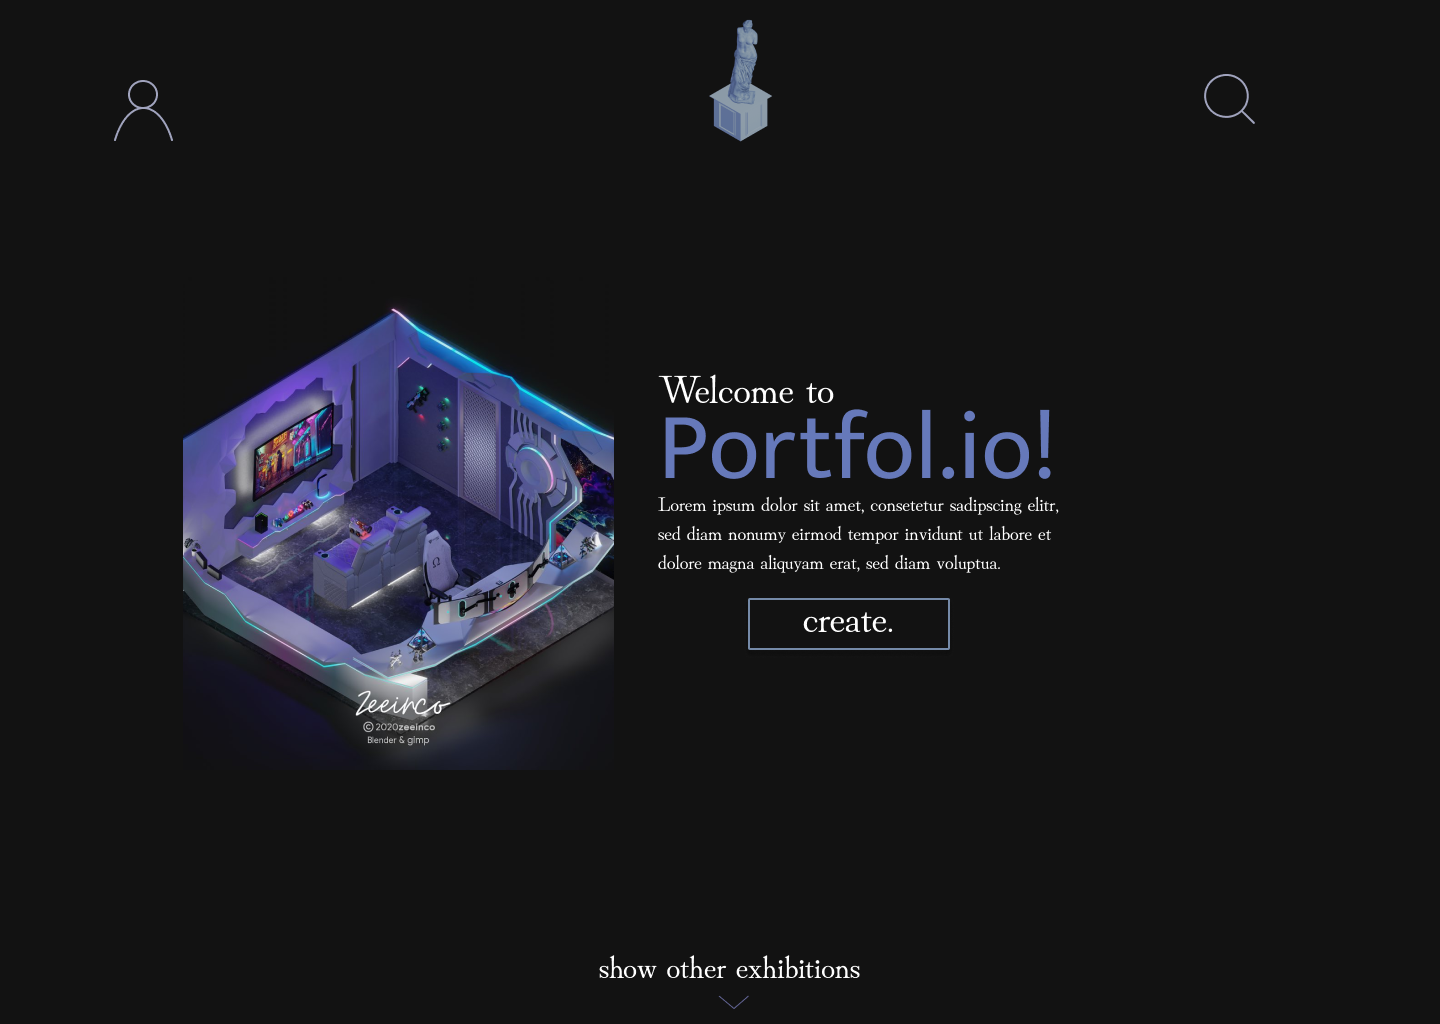
\includegraphics[scale=0.3]{pics/DesignKonzept1_1.png}
    \caption{Design Konzpet 1 Page 1}
    \label{fig:impl:knuth}
\end{figure}

\begin{figure}
    \centering
    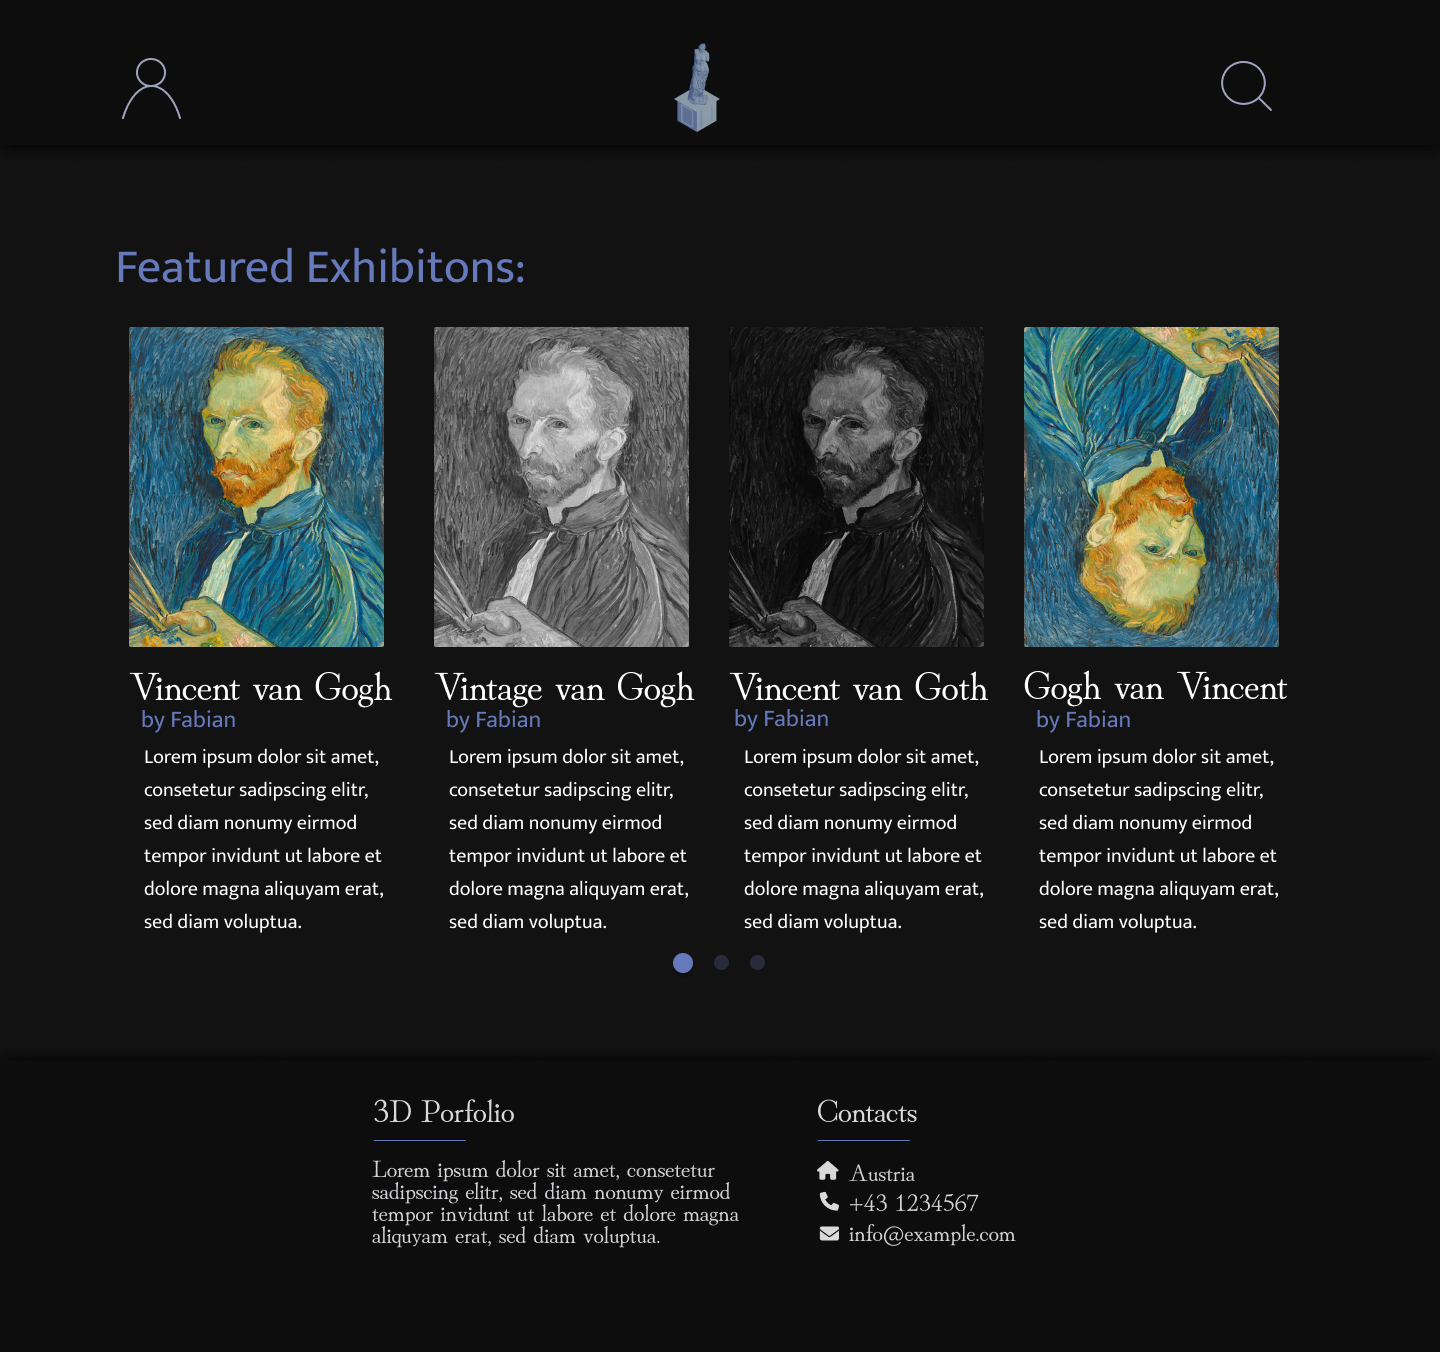
\includegraphics[scale=0.3]{pics/DesignKonzept1_2.png}
    \caption{Design Konzpet 1 Page 2}
    \label{fig:impl:knuth}
\end{figure}

\begin{figure}
    \centering
    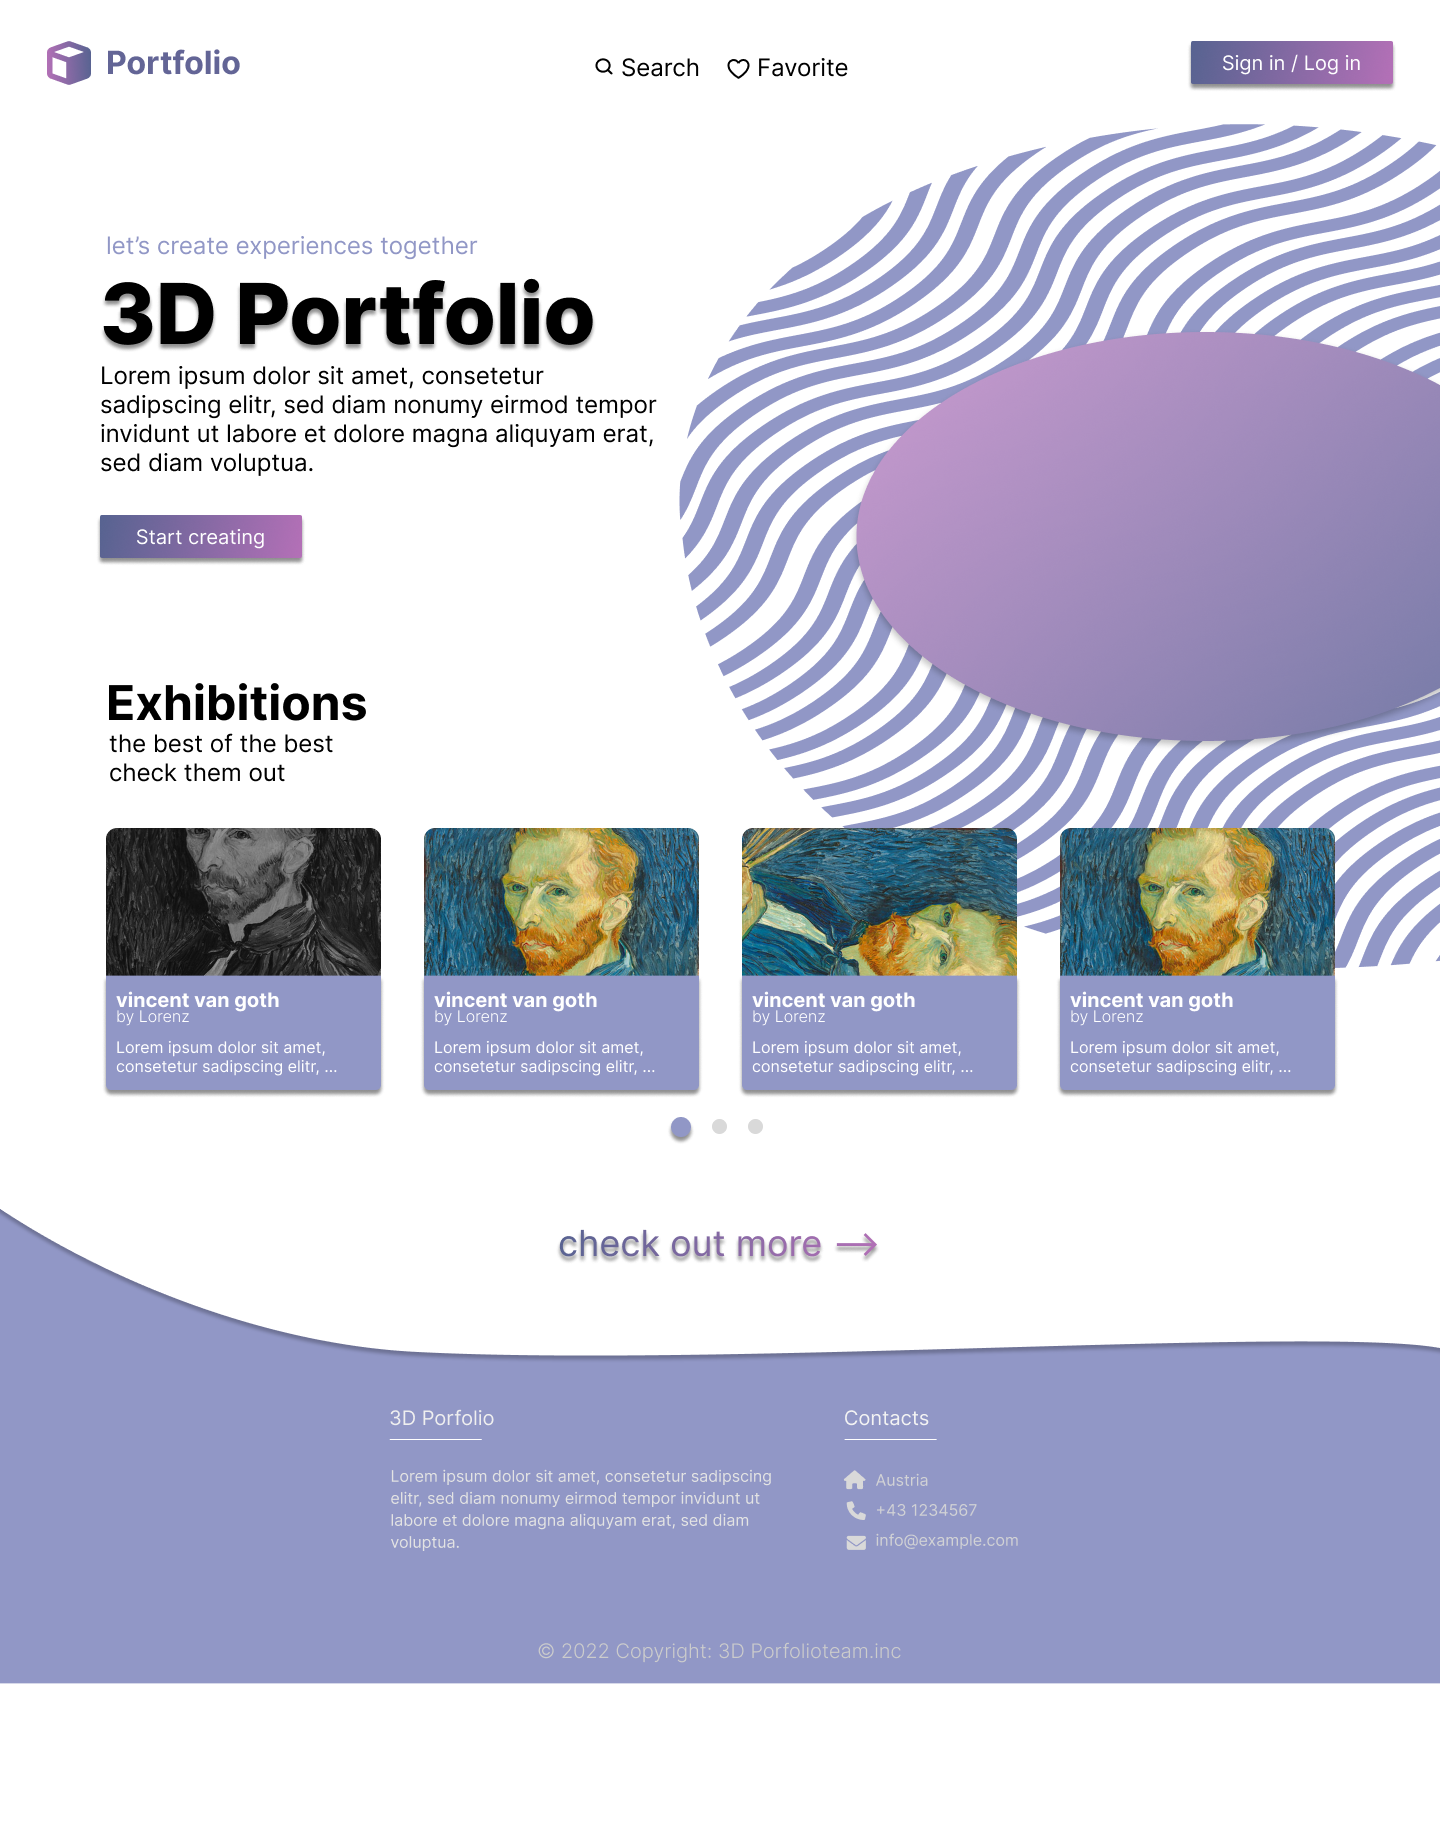
\includegraphics[scale=0.3]{pics/DesignKonzept2.png}
    \caption{Design Konzept 2}
    \label{fig:impl:knuth}
\end{figure}

